\section{Experimental Design}

Our experimental design systematically tests the central thesis that selective layer aggregation can preserve distinct playstyles while maintaining competitive playing strength. We employ a multi-phase approach comprising baseline experiments (establishing bounds on knowledge sharing), selective aggregation experiments (testing different layer sharing strategies), and performance evaluation experiments (validating playstyle preservation and generalization). The complete experimental matrix is presented in Figure~\ref{fig:experiment-matrix}.

\begin{figure}[htbp]
\centering
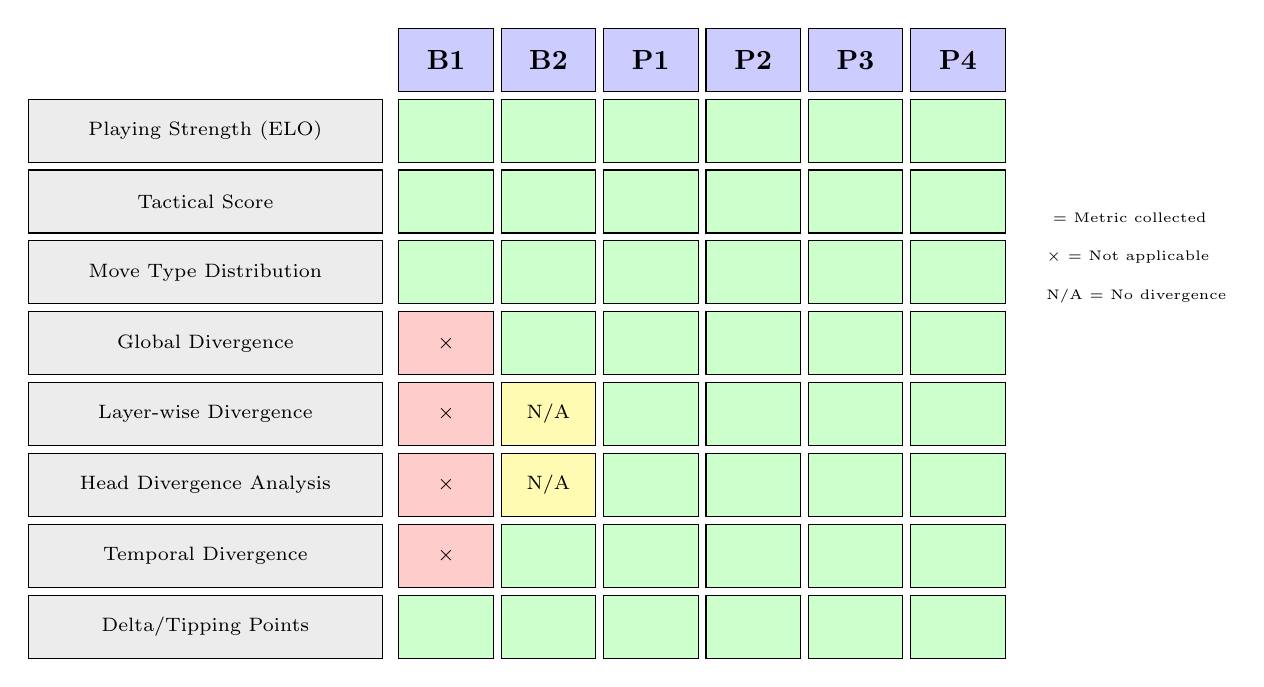
\begin{tikzpicture}[
    scale=1,
    transform shape,
    cell/.style={rectangle, draw=black, minimum width=1.2cm, minimum height=0.8cm, font=\scriptsize, align=center},
    header/.style={rectangle, draw=black, fill=blue!20, minimum width=1.2cm, minimum height=0.8cm, font=\scriptsize, align=center, font=\bfseries},
    rowlabel/.style={rectangle, draw=black, fill=gray!15, minimum width=4.5cm, minimum height=0.8cm, font=\scriptsize, align=center},
]

% Column headerss
\node[header] at (0, 0) {B1};
\node[header] at (1.3, 0) {B2};
\node[header] at (2.6, 0) {P1};
\node[header] at (3.9, 0) {P2};
\node[header] at (5.2, 0) {P3};
\node[header] at (6.5, 0) {P4};

% Row labels and cells
\node[rowlabel, anchor=east] at (-0.8, -0.9) {Playing Strength (ELO)};
\node[cell, fill=green!20] at (0, -0.9) {$\checkmark$};
\node[cell, fill=green!20] at (1.3, -0.9) {$\checkmark$};
\node[cell, fill=green!20] at (2.6, -0.9) {$\checkmark$};
\node[cell, fill=green!20] at (3.9, -0.9) {$\checkmark$};
\node[cell, fill=green!20] at (5.2, -0.9) {$\checkmark$};
\node[cell, fill=green!20] at (6.5, -0.9) {$\checkmark$};

\node[rowlabel, anchor=east] at (-0.8, -1.8) {Tactical Score};
\node[cell, fill=green!20] at (0, -1.8) {$\checkmark$};
\node[cell, fill=green!20] at (1.3, -1.8) {$\checkmark$};
\node[cell, fill=green!20] at (2.6, -1.8) {$\checkmark$};
\node[cell, fill=green!20] at (3.9, -1.8) {$\checkmark$};
\node[cell, fill=green!20] at (5.2, -1.8) {$\checkmark$};
\node[cell, fill=green!20] at (6.5, -1.8) {$\checkmark$};

\node[rowlabel, anchor=east] at (-0.8, -2.7) {Move Type Distribution};
\node[cell, fill=green!20] at (0, -2.7) {$\checkmark$};
\node[cell, fill=green!20] at (1.3, -2.7) {$\checkmark$};
\node[cell, fill=green!20] at (2.6, -2.7) {$\checkmark$};
\node[cell, fill=green!20] at (3.9, -2.7) {$\checkmark$};
\node[cell, fill=green!20] at (5.2, -2.7) {$\checkmark$};
\node[cell, fill=green!20] at (6.5, -2.7) {$\checkmark$};

\node[rowlabel, anchor=east] at (-0.8, -3.6) {Global Divergence};
\node[cell, fill=red!20] at (0, -3.6) {$\times$};
\node[cell, fill=green!20] at (1.3, -3.6) {$\checkmark$};
\node[cell, fill=green!20] at (2.6, -3.6) {$\checkmark$};
\node[cell, fill=green!20] at (3.9, -3.6) {$\checkmark$};
\node[cell, fill=green!20] at (5.2, -3.6) {$\checkmark$};
\node[cell, fill=green!20] at (6.5, -3.6) {$\checkmark$};

\node[rowlabel, anchor=east] at (-0.8, -4.5) {Layer-wise Divergence};
\node[cell, fill=red!20] at (0, -4.5) {$\times$};
\node[cell, fill=yellow!30] at (1.3, -4.5) {N/A};
\node[cell, fill=green!20] at (2.6, -4.5) {$\checkmark$};
\node[cell, fill=green!20] at (3.9, -4.5) {$\checkmark$};
\node[cell, fill=green!20] at (5.2, -4.5) {$\checkmark$};
\node[cell, fill=green!20] at (6.5, -4.5) {$\checkmark$};

\node[rowlabel, anchor=east] at (-0.8, -5.4) {Head Divergence Analysis};
\node[cell, fill=red!20] at (0, -5.4) {$\times$};
\node[cell, fill=yellow!30] at (1.3, -5.4) {N/A};
\node[cell, fill=green!20] at (2.6, -5.4) {$\checkmark$};
\node[cell, fill=green!20] at (3.9, -5.4) {$\checkmark$};
\node[cell, fill=green!20] at (5.2, -5.4) {$\checkmark$};
\node[cell, fill=green!20] at (6.5, -5.4) {$\checkmark$};

\node[rowlabel, anchor=east] at (-0.8, -6.3) {Temporal Divergence};
\node[cell, fill=red!20] at (0, -6.3) {$\times$};
\node[cell, fill=green!20] at (1.3, -6.3) {$\checkmark$};
\node[cell, fill=green!20] at (2.6, -6.3) {$\checkmark$};
\node[cell, fill=green!20] at (3.9, -6.3) {$\checkmark$};
\node[cell, fill=green!20] at (5.2, -6.3) {$\checkmark$};
\node[cell, fill=green!20] at (6.5, -6.3) {$\checkmark$};

\node[rowlabel, anchor=east] at (-0.8, -7.2) {Delta/Tipping Points};
\node[cell, fill=green!20] at (0, -7.2) {$\checkmark$};
\node[cell, fill=green!20] at (1.3, -7.2) {$\checkmark$};
\node[cell, fill=green!20] at (2.6, -7.2) {$\checkmark$};
\node[cell, fill=green!20] at (3.9, -7.2) {$\checkmark$};
\node[cell, fill=green!20] at (5.2, -7.2) {$\checkmark$};
\node[cell, fill=green!20] at (6.5, -7.2) {$\checkmark$};

% Legend
\node[font=\tiny, anchor=west] at (7.5, -2) {$\checkmark$ = Metric collected};
\node[font=\tiny, anchor=west] at (7.5, -2.5) {$\times$ = Not applicable};
\node[font=\tiny, anchor=west] at (7.5, -3) {N/A = No divergence};

\end{tikzpicture}
\caption{Experimental design matrix showing which metrics are collected for each experiment configuration. B1 (Full Sharing) and B2 (No Sharing) establish baseline bounds, while P1-P4 test selective aggregation strategies. All configurations measure playing strength and playstyle characteristics; divergence metrics are only meaningful where clusters can diverge.}
\label{fig:experiment-matrix}
\end{figure}

\subsection{Baseline Experiments}

The baseline experiments establish the performance bounds for our system, demonstrating what happens under extreme aggregation policies: full knowledge sharing (all layers aggregated) versus zero knowledge sharing (independent cluster training). These baselines provide reference points for evaluating selective aggregation strategies.

\subsubsection{B1: Full Sharing Baseline}

The full sharing baseline (B1) implements standard federated averaging across all network layers, providing a control configuration that demonstrates the effects of complete knowledge transfer without any selective aggregation. In this configuration, both tactical and positional clusters participate in global aggregation at every round, with all layer groups (input block, all 19 residual blocks, policy head, value head) averaged across clusters using the FedAvg algorithm.

This baseline tests the hypothesis that standard federated learning, while effective at leveraging collective training data, destroys cluster-specific patterns that encode distinct playstyles. We expect clusters to converge toward identical representations as all parameters are continuously averaged, eliminating any divergence that might otherwise develop through playstyle-specific training data. The tactical and positional clusters should exhibit minimal playstyle separation, with tactical scores converging to approximately 0.5-0.6 (balanced play) regardless of the training data filtering.

Training configuration for B1 uses 200 rounds with 4 clients per cluster, each processing 400 games per round from their respective playstyle-filtered datasets. Despite the data filtering (tactical cluster trains on tactical puzzles, positional cluster trains on endgame/positional puzzles), the continuous averaging of all network parameters should prevent clusters from developing and maintaining distinct internal representations corresponding to their training data characteristics.

Expected outcomes for B1 include near-zero global divergence (cosine similarity exceeding 0.99 across all layers), minimal playstyle separation between clusters (tactical score difference less than 0.1), and moderate ELO performance (approximately 1300-1500) reflecting the benefits of aggregating knowledge from both clusters while potentially suffering from conflicting gradient updates due to the different training objectives.

\subsubsection{B2: No Sharing Baseline}

The no sharing baseline (B2) represents the opposite extreme: complete independence between clusters with no inter-cluster communication. Each cluster performs intra-cluster aggregation using FedAvg to combine knowledge from its 4 constituent clients, but clusters never exchange parameters with each other. This configuration establishes the maximum possible divergence achievable when clusters independently optimize for their respective playstyle-specific training data.

This baseline tests whether independent training on playstyle-filtered data is sufficient to produce measurable and consistent playstyle differences, and quantifies the performance cost (if any) of forgoing knowledge transfer between clusters. We expect B2 to show the highest divergence across all layer groups, with clusters developing completely independent representations optimized for their respective tactical or positional training objectives.

The training configuration for B2 mirrors B1 (200 rounds, 4 clients per cluster, 400 games per round), but aggregation is strictly limited to within-cluster averaging. The tactical cluster aggregates only among tactical clients, and the positional cluster aggregates only among positional clients. This effectively divides the system into two independent federated learning deployments operating on different training data distributions.

Expected outcomes for B2 include maximum global divergence (cosine similarity potentially dropping below 0.7 for policy and value heads), strong playstyle separation (tactical scores diverging by 0.20 or more between clusters with tactical cluster exceeding 0.65 and positional cluster below 0.50), and potentially lower individual cluster ELO (approximately 1200-1400) due to the reduced effective training data compared to configurations that share knowledge. The B2 baseline demonstrates the upper bound on playstyle preservation at the potential cost of playing strength.

\subsection{Selective Aggregation Experiments}

The selective aggregation experiments (P1-P4) constitute the core empirical contribution of this work, testing different hypotheses about where in the neural network architecture playstyle-specific versus general chess knowledge resides. Each configuration selectively shares different layer groups while keeping others cluster-specific, enabling us to identify which layers benefit from sharing (universal chess patterns) and which should remain independent (playstyle-specific representations).

\subsubsection{P1: Share Early Layers Only}

Configuration P1 tests the hypothesis that early network layers learn general chess features (piece recognition, basic board patterns, elementary tactical motifs) that are universal across playstyles and thus benefit from sharing, while late layers and output heads encode playstyle-specific strategic preferences that should diverge.

In P1, the shared layer groups comprise the input block (input convolution and batch normalization) and early residual blocks (residual layers 0-5), totaling approximately 2.5 million parameters representing roughly 11\% of the network. These layers process raw board representations and extract low-level features such as piece positions, material balance, and simple tactical patterns (attacks, defenses, pins).

The cluster-specific layer groups include middle residual blocks (layers 6-12), late residual blocks (layers 13-18), policy head, and value head, representing approximately 8.5 million parameters (38\% of the network). These layers synthesize low-level features into strategic understanding and decision-making, where we hypothesize that tactical versus positional distinctions emerge.

Expected outcomes for P1 include shared early layers showing near-zero divergence (cosine similarity above 0.98) while cluster-specific layers exhibit increasing divergence with network depth, potentially reaching divergence indices of 0.5-0.8 in the policy head. We expect moderate playstyle separation (tactical score difference of 0.15-0.20) and good playing strength (ELO 1400-1600) as clusters benefit from shared foundational features while specializing their decision-making.

This configuration directly tests hypothesis H3 (early layers remain shared while late layers diverge) by explicitly enforcing this structure through the aggregation policy. Analysis of layer-wise divergence should reveal a clear gradient from low divergence in shared early blocks to high divergence in cluster-specific late blocks.

\subsubsection{P2: Share Middle Layers Only}

Configuration P2 represents an exploratory experiment testing the counter-intuitive hypothesis that mid-level tactical pattern recognition (forks, pins, skewers, discovered attacks) might be universal across playstyles, benefiting from shared representations, while low-level feature extraction and high-level strategic planning should remain cluster-specific.

In P2, only the middle residual blocks (layers 6-12) are shared between clusters, representing approximately 3.5 million parameters. These middle layers operate on features extracted by the (cluster-specific) input and early blocks, detecting intermediate-level patterns such as piece coordination, tactical motifs, and local threats. All other layer groups, input block, early residual blocks, late residual blocks, and both output heads, remain cluster-specific.

This configuration produces an unusual divergence signature: high divergence at the input (cluster-specific feature extraction), low divergence in the middle (shared tactical patterns), and high divergence at the output (cluster-specific strategic synthesis). If the hypothesis holds, we should observe that sharing middle layers improves both clusters' ability to recognize tactical opportunities, even though they apply this recognition differently based on their cluster-specific strategic frameworks.

Expected outcomes for P2 are less certain than for other configurations, as this is primarily an exploratory experiment to understand layer roles. We anticipate moderate divergence in input and early layers (divergence index 0.3-0.5), low divergence in middle layers (cosine similarity above 0.95), and high divergence in late layers and heads (divergence index 0.6-1.0). Playstyle separation may be lower than B2 but higher than B1 (tactical score difference 0.10-0.15), and playing strength should be moderate (ELO 1350-1500).

\subsubsection{P3: Share Late Layers and Heads}

Configuration P3 serves as a control experiment testing the inverse hypothesis to P1: that high-level strategic reasoning is universal across playstyles while low-level feature extraction is playstyle-specific. We include P3 primarily to validate (through expected failure) that output heads must remain cluster-specific to encode distinct move preferences.

In P3, the shared layer groups comprise late residual blocks (layers 13-18), policy head, and value head, totaling approximately 5.5 million parameters. These layers perform strategic synthesis and decision-making. The cluster-specific layers include the input block, early residual blocks (0-5), and middle residual blocks (6-12), representing the feature extraction and pattern detection stages of the network.

We expect P3 to show poor performance on playstyle preservation metrics, as sharing the policy head forces both clusters to make similar move selections despite training on different data distributions. The shared policy head must compromise between tactical and positional preferences, likely resulting in middling play that satisfies neither cluster's training objective well.

Expected outcomes include low divergence in shared late layers and heads (by construction), higher divergence in cluster-specific early/middle layers, minimal playstyle separation (tactical score difference less than 0.08), and relatively low playing strength (ELO 1250-1400) as the shared decision-making heads cannot specialize for either playstyle. This configuration validates hypothesis H4 (policy head divergence is necessary for playstyle expression) through its anticipated failure.

\subsubsection{P4: Share Backbone, Separate Heads}

Configuration P4 tests what we hypothesize is the optimal selective aggregation strategy: share the entire residual backbone (all feature extraction and pattern recognition layers) while keeping only the output heads cluster-specific. This configuration embodies the principle that chess features are largely universal, but their application to move selection (policy) and position evaluation (value) depends on playstyle preferences.

In P4, the shared layer groups comprise the input block and all 19 residual blocks, totaling approximately 20 million parameters (87\% of the network). These layers learn piece recognition, tactical pattern detection, strategic concept representation, and deep positional understanding. The cluster-specific layer groups include only the policy head and value head (approximately 2 million parameters, 9\% of the network).

This configuration enables maximum knowledge transfer, both clusters benefit from a shared, rich representation of chess positions developed through training on the combined dataset of tactical and positional games. However, the cluster-specific heads translate this shared representation into cluster-appropriate decisions: the tactical cluster's policy head learns to prioritize forcing moves, sacrifices, and direct attacks, while the positional cluster's policy head learns to prioritize pawn structure, piece coordination, and long-term advantages.

Expected outcomes for P4 include near-zero divergence across the entire backbone (cosine similarity exceeding 0.99 for all residual blocks), high divergence in the policy head (divergence index 0.7-1.2 as clusters learn fundamentally different move preferences), moderate divergence in the value head (divergence index 0.4-0.7 as evaluation criteria differ but share common factors like material and king safety), strong playstyle separation (tactical score difference 0.18-0.25), and the highest playing strength among all configurations (ELO 1500-1700) due to maximum knowledge sharing combined with playstyle specialization.

P4 directly addresses research questions about where playstyles are encoded (primarily in output heads) and whether knowledge transfer and playstyle diversity are compatible objectives (yes, through selective head specialization).

\subsection{Research Hypotheses and Validation}

Our experimental design tests five primary hypotheses and five secondary hypotheses regarding selective aggregation, playstyle preservation, and knowledge transfer in federated deep reinforcement learning.

\subsubsection{Primary Hypotheses}

\textbf{H1: Selective aggregation preserves playstyles better than full aggregation.} We validate H1 by comparing playstyle divergence (standard deviation of tactical scores across clusters) between P1-P4 and the B1 baseline. Success requires that at least one selective configuration (we hypothesize P4) achieves significantly higher playstyle divergence than B1 (two-sample t-test, $p < 0.05$), with tactical score differences exceeding 0.15 compared to B1's expected difference of less than 0.10.

\textbf{H2: Full aggregation destroys cluster-specific patterns.} We validate H2 through layer-wise divergence analysis of B1, demonstrating that continuous averaging of all parameters prevents divergence from developing. Success requires that B1 shows uniformly low divergence (cosine similarity $> 0.95$) across all layer groups throughout training, even though clusters train on playstyle-filtered data.

\textbf{H3: Early layers remain shared while late layers diverge.} We validate H3 by analyzing per-layer-group divergence in P1-P4, particularly P1 which explicitly tests this structure. Success requires observing a clear layer-depth gradient: shared layers maintain high cosine similarity ($> 0.95$), cluster-specific layers develop significant divergence (cosine similarity $< 0.85$ for policy head), with intermediate layers showing intermediate divergence if they are cluster-specific.

\textbf{H4: Policy head diverges more than value head.} We validate H4 by comparing divergence indices for policy and value heads across P1, P2, and P4 (configurations where both heads are cluster-specific). Success requires that policy head divergence exceeds value head divergence by at least 20\% (e.g., policy divergence index 0.8 vs.~value divergence index 0.6), reflecting stronger playstyle-specific patterns in move selection than in position evaluation.

\textbf{H5: Divergence increases then plateaus during training.} We validate H5 through temporal divergence analysis, tracking mean divergence across cluster-specific layers over 200 training rounds. Success requires detecting a plateau phase where divergence velocity (change per 10 rounds) approaches zero, typically occurring between rounds 80-120, indicating that clusters have settled into stable distinct representations constrained by the selective aggregation policy.

\subsubsection{Secondary Hypotheses}

\textbf{H6: Tactical cluster develops preference for aggressive moves.} We validate H6 through move type distribution analysis, comparing captures percentage, checks percentage, and aggressive moves percentage between clusters. Success requires that the tactical cluster shows statistically significantly higher rates (two-sample t-test, $p < 0.01$) for these categories, with captures percentage exceeding the positional cluster by at least 3 percentage points.

\textbf{H7: Positional cluster develops preference for quiet, strategic moves.} We validate H7 similarly to H6, testing whether the positional cluster shows significantly higher pawn advances percentage and quiet moves percentage. Success requires the positional cluster to exceed the tactical cluster by at least 5 percentage points in quiet moves and 4 percentage points in pawn advances.

\textbf{H8: Both clusters maintain competitive playing strength.} We validate H8 by requiring that both clusters achieve ELO ratings above 1400 in the best-performing selective aggregation configuration (hypothesized to be P4). This threshold represents intermediate-level chess ability and demonstrates that playstyle preservation does not come at the cost of basic playing competence.

\textbf{H9: Model divergence correlates with playstyle divergence.} We validate H9 by computing Pearson correlation between global divergence index (mean across all cluster-specific layers) and tactical score difference (absolute difference in mean tactical scores) across all configurations and training rounds. Success requires positive correlation ($r > 0.6$, $p < 0.001$), indicating that parameter-level differences correspond to behavioral differences.

\textbf{H10: Shared layers enable knowledge transfer.} We validate H10 by comparing learning curves (ELO over training rounds) between B2 (no sharing) and P1-P4 (selective sharing). Success requires that selective aggregation configurations achieve target ELO values in fewer rounds than B2, demonstrating accelerated learning through knowledge transfer from shared layers.

\subsection{Experimental Parameters and Logistics}

All experiments use identical base training parameters to ensure fair comparison. Each cluster consists of 4 clients, with training proceeding for 200 rounds. Each client processes 400 games per round from its playstyle-specific filtered dataset (tactical clients use tactical puzzles, positional clients use positional puzzles). Batch size is 64, initial learning rate is 0.003 with ReduceLROnPlateau scheduling (factor 0.5, patience 15 rounds, minimum learning rate $10^{-6}$).

Evaluation occurs every 10 rounds, generating 30 games per cluster against Stockfish opponents at ELO levels 1000, 1200, and 1400 (10 games per level with alternating colors). Each evaluation game is analyzed to extract tactical scores, move type distributions, delta metrics, and all other playstyle characteristics described in Section~\ref{sec:evaluation}. Model divergence metrics are computed every 10 rounds by loading both cluster models and performing layer-wise weight comparisons.

The complete experimental timeline spans approximately 6-8 weeks: Phase 1 (baselines B1 and B2) requires 4-5 days of training plus 2-3 days of analysis, Phase 2 (selective aggregation P1-P4) requires 20-25 days of training plus 5-7 days of analysis, and Phase 3 (final performance evaluation and generalization tests) requires 3-5 days. Total computational requirements are approximately 1000-1200 GPU hours on NVIDIA RTX 3090 or equivalent hardware with 24GB VRAM.

